% !TEX root = main.tex
\label{sec:background}
\begin{figure*}[t]
\centering
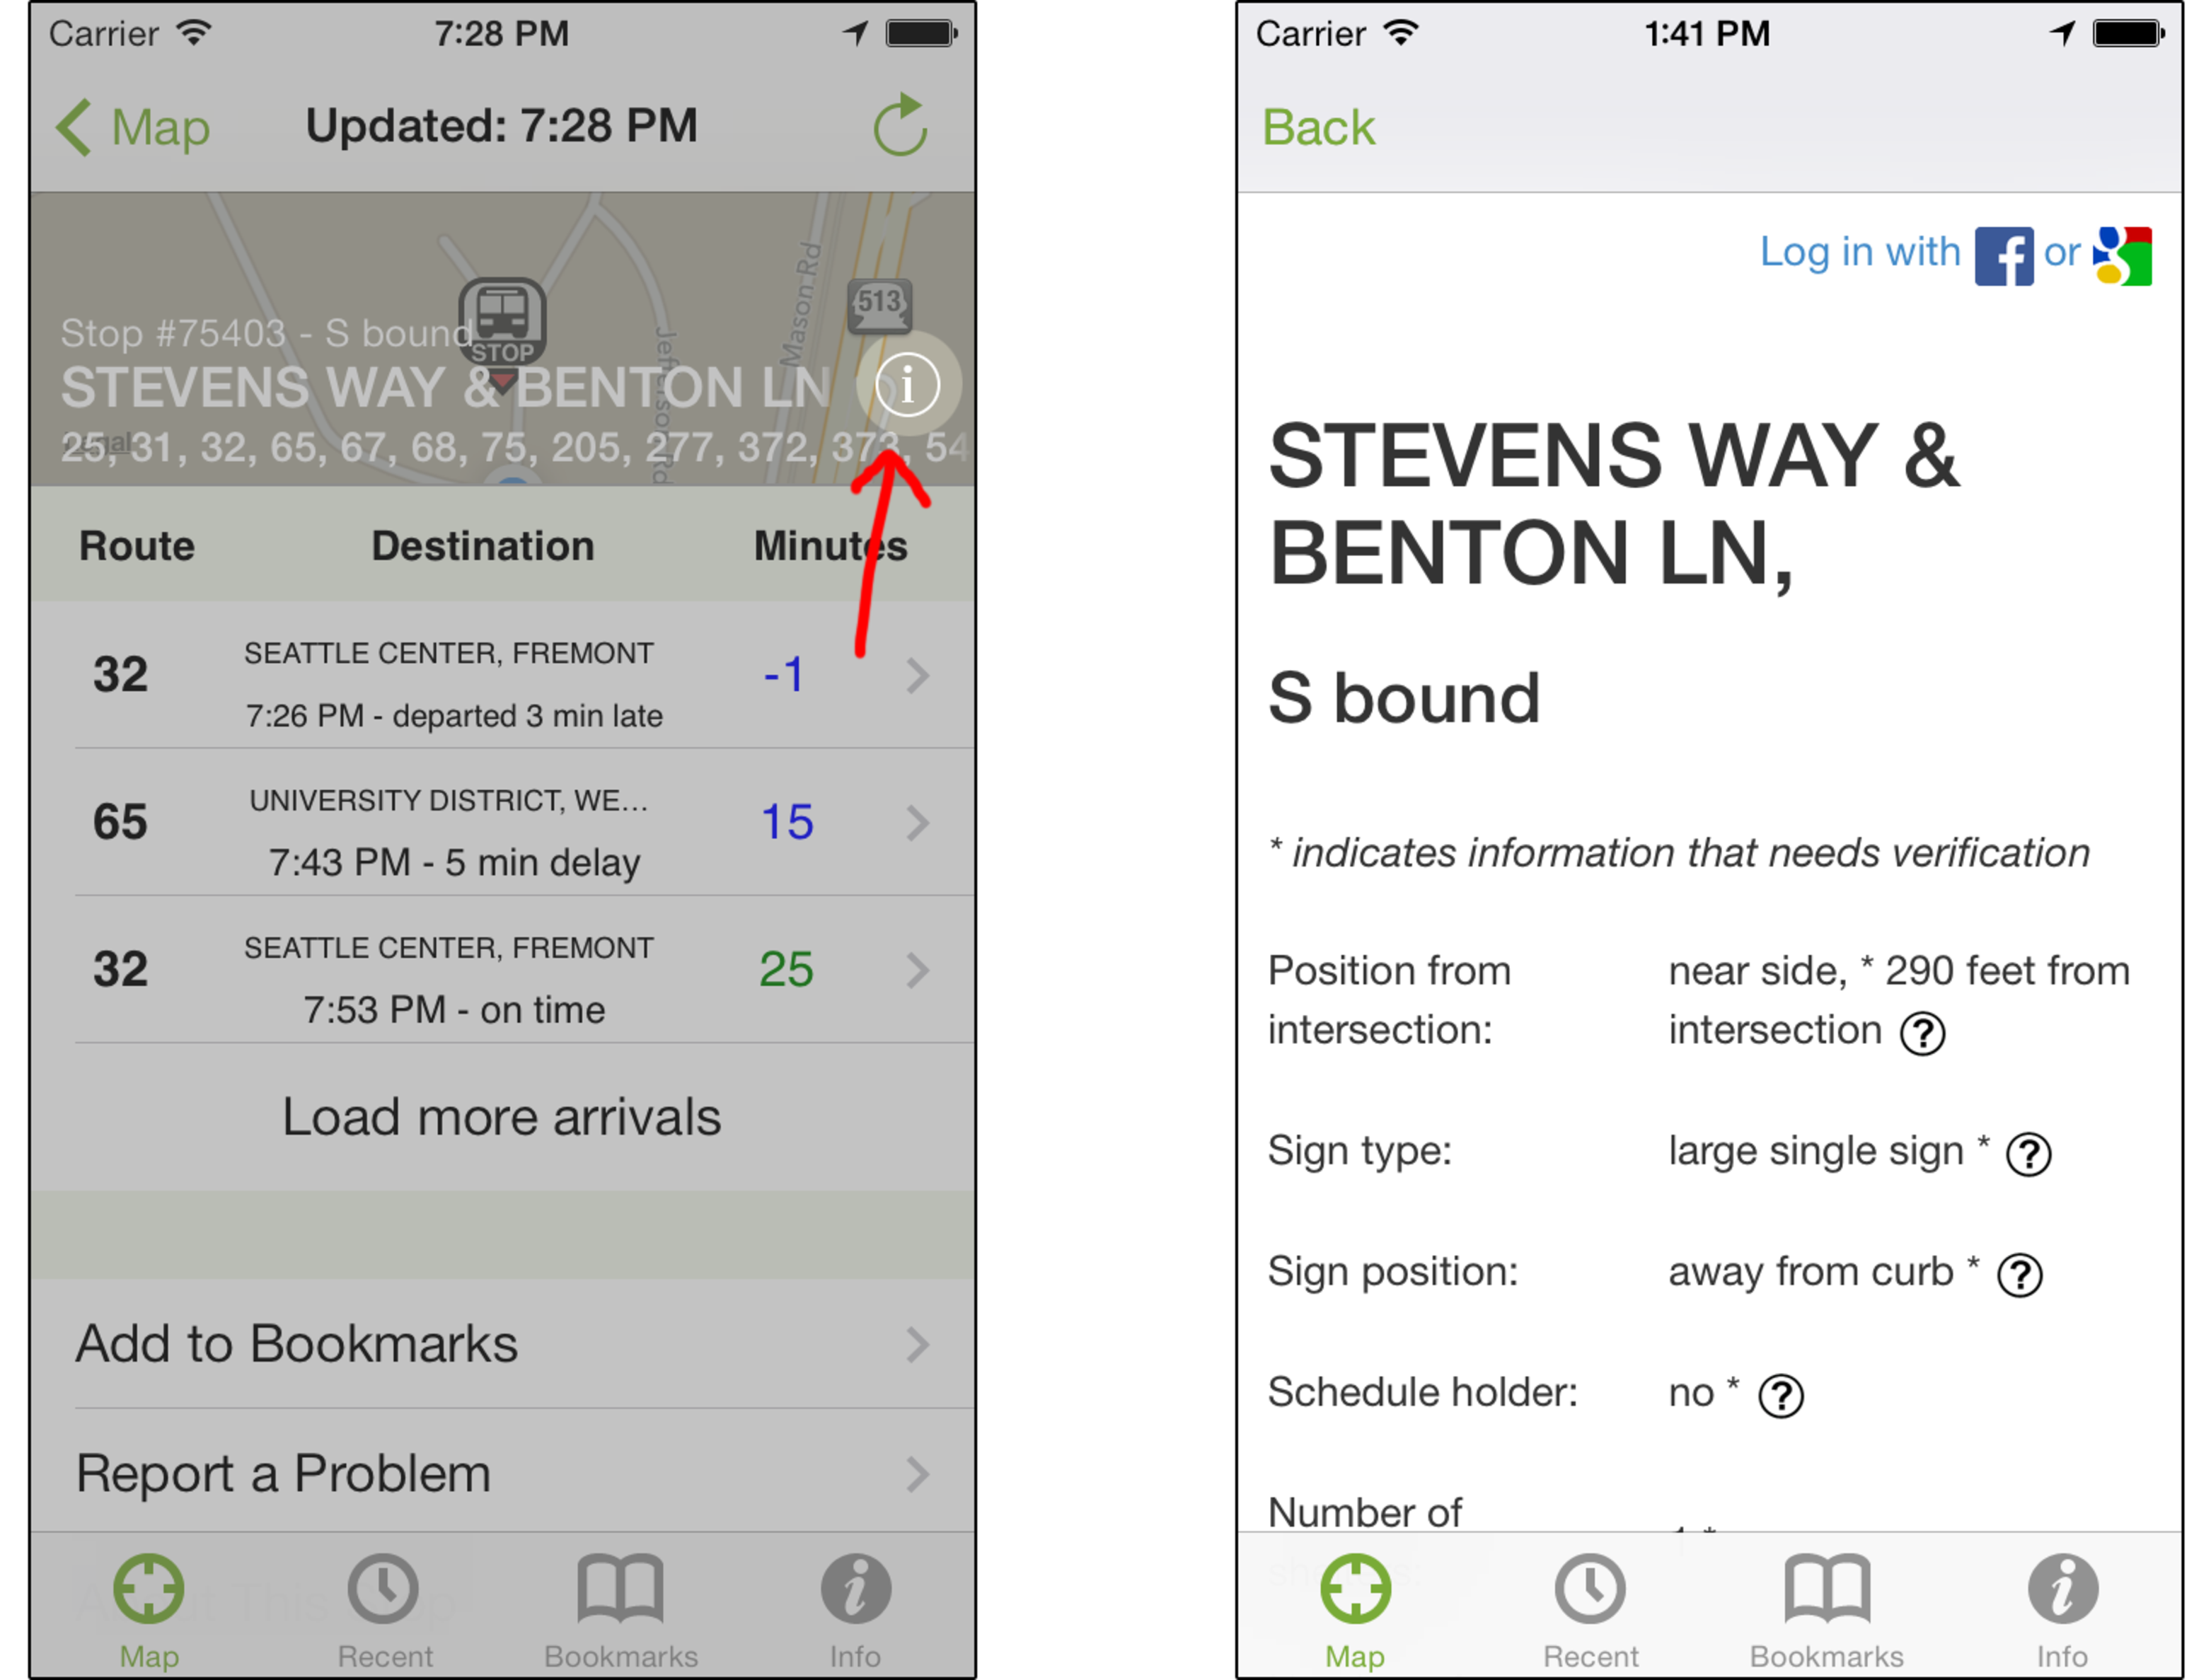
\includegraphics[width=.60\textwidth]{StopInfoAppScreen.pdf}
\caption{(left) The stop details screen in OneBusAway. StopInfo can be
accessed through the info button next to the title. (right) The StopInfo
view and associated information for the specified stop. An asterisk
next to a field means that information has not yet been verified by three 
or more people. If no information exists for a particular field, we do not
display it.  Both screens were also tested extensively for
accessibility using VoiceOver.}
\label{fig:app-screen}
\end{figure*} 

\section{The StopInfo System}

\subsection{OneBusAway}
StopInfo is a web-based application that has been incorporated into OneBusAway \cite{ferris-phd, watkins-phd},
a set of tools that provide real-time arrival
predictions and other transit information, such as where bus stops
are located on a map and which stops are traversed by a particular
route. OneBusAway builds on the work of Dan Dailey and others on real-time transit 
information systems, such as MyBus and BusView \cite{maclean-trb-2002}, and has been widely 
adopted in the Puget Sound region, used by over 100,000 unique transit riders each week. The system is freely available as an application on the iOS, Android, and 
Windows Phone platforms, and also via SMS, interactive voice response, and the 
Web. Research on OneBusAway has found a number of significant 
benefits, including increased or greatly increased satisfaction with public 
transit for 92\% of survey respondents, increased feelings of safety for some
(particularly while waiting at night), and decreased wait time at the stop
\cite{watkins-transportation-research-2011}.  One of the goals of our research 
group is to make these benefits available to as wide a range of people 
as possible, and we have devoted significant attention to ensuring that the
apps, in particular the iOS app, provide adequate accessibility.

We decided to integrate StopInfo with OneBusAway on iOS for a number
of reasons. First, OneBusAway is already used by a large number of
people, and many check the application from their smartphones while 
waiting at bus stops. This enables us to leverage a large existing user base by directly allowing the community to enter information for the stop as they 
wait. Secondly, the OneBusAway iOS application is already heavily used 
by members of the blind, low vision, and 
deaf-blind communities in the greater Seattle region who use and rely on
public transit, and has been developed and tested to remain
accessible to this community. Finally, StopInfo is a natural extension of 
OneBusAway, and can also be useful to
the general population of transit riders. It includes relevant information such 
as how well-lit a stop is at night, which has safety implications, and whether
a stop may be closed.

We integrated StopInfo with OneBusAway iOS by placing an info button with the
accessibility label ``About This Stop'' next to the name of the stop on the 
details view for that stop (Figure \ref{fig:app-screen}).  Tapping or double tapping 
on the button brings up StopInfo as an integrated
web view within the application, and is also accessible to people with visual impairments through Apple's
VoiceOver screen reader. 

\pagebreak

\subsection{StopInfo Interface}
When a user accesses StopInfo, they are presented with a text list of the stop features.  
An asterisk next an item of information indicates that the information still needs verification from at least two more people.

Below the list of stop information there are links to add or verify information,
report a stop closure, or access some frequently asked questions. In the top right corner of the screen, there is an option to sign in with an existing Facebook or Google account. 

To help encourage contributions, five months after our initial launch of StopInfo, we introduced a reputation system that allows users who are signed in to earn points and badges by entering stop information. They can also make it onto a ``top contributors'' list if they choose to display their profile publicly and if they are among the top twenty users points-wise. For a short time, we also offered the top information contributors free bus passes provided by King County Metro as potential rewards. 

\subsection{Accuracy and Completeness of Information in StopInfo}

In an initial audit conducted two to three months into the deployment of StopInfo, we found that the information submitted by contributors was largely accurate for most categories (the categories that were less accurate were due to ambiguities on our part, which we have since improved) \cite{campbell-2014}. Another accuracy audit is soon forthcoming, which will inform us of any other potential ambiguities or undesired behaviors in the system (however, we have been manually monitoring submissions and have thus far not noticed malicious or gaming behaviors). 

In terms of completeness, out of the 8,481 total bus stops in our system, we have basic information (the position of stop relative to the intersection, the number of shelters, and the type of sign) for all of them, since it was provided by King County Metro. Additionally, StopInfo contributors have added information for categories not provided by the transit agency for 1,148 stops (or 13.5\% of the total stops covered by King County Metro). Each of these stops received one to two submissions on average (of course, some have many more submissions depending on how frequently that stop is accessed). While we are happy with that number, we believe we can do better in terms of breadth by incentivizing people to contribute to stops they do not normally frequent (or extending access and awareness of StopInfo to certain areas). Possible incentives for encouraging breadth will be discussed in a later section.
